\chapter{Tecniche che fanno uso di altri segnali}
 Come già discusso nei capitoli precedenti, le tecniche basate sul contenuto utilizzano delle feature determinate empiricamente su alcuni dataset di pagine web a disposizione dei ricercatori mentre le tecniche che basate sul grafo diminuiscono o eliminano del tutto l'impatto dello score dei nodi spam attraverso la determinazione di alcuni pattern strutturali all'interno del grafo.  Le tecniche che vengono descritti in questo capitolo sono la risposta alla continua evoluzione delle tecniche di web spam; Tali tecniche utilizzano come segnale di partenza oggetti al di fuori del contenuto delle pagine web e della struttura del grafo. Questi nuovi tipi di approccio sono stati sviluppati per identificare tutti i vari tipi di spam che hanno caratteristiche tali da non essere identificabili con i metodi tradizionali oppure quando si voglia usarle in modo complementare alle tecniche già presenti in letteratura. 


\section{Rilevamento dello spam di tipo cloaking}
Ci sono pochi metodi che tentano di rilevare il cloaking. Gli spammer possono rilevare un crawler dal suo indirizzo IP o dal campo \textit{user-agent} all'interno di una richiesta HTTP e quindi fornire due versioni di una pagina a seconda di chi effettui la richiesta. Molti dei metodi per rilevare il cloaking prendono in considerazioni due copie di una stessa pagina, la prima è ottenuta tramite un richiesta HTTP al server (proprietario della pagina) da parte di un crawler mentre la seconda è ottenuta tramite la richiesta HTTP al server da parte di un browser; le due copie vengono quindi confrontate per verificare se siano identiche e escludere che si tratti di cloaking. Tuttavia tali metodi non sono efficaci in quanto con l'avvento del WEB 2.0 le pagine vengono generate dinamicamente e possono variare nei contenuti. Per superare l'incertezza legata alla natura dinamica delle pagine si può utilizzare un metodo \cite{Ghiam:2013cloaking} che si basa sul confronto dei termini tra le due copie di una pagina 
usando delle funzioni hash per aumentare la velocità di confronto. Il metodo definisce  \(C_i\) l'insieme delle copie di una pagina che sono ottenute tramite le richieste fatte da parte di un crawler al server, \(B_i\) l'insieme delle copie di una pagina che sono conseguite attraverso delle richieste da parte di un browser al server e \(f\) una funzione di hash che viene applicata alle copie ottenute \(B_i\) e \(C_i\); se i valori di hash ottenuti dalle copie del browser e del crawler  sono identici  ne consegue che  le pagine sono identiche, viceversa le due pagine sono differenti. L'algoritmo differenzia il cloaking in statico e dinamico. Nel primo caso ci si trova nella situazione in cui le copie di una pagina del browser e del crawler sono diverse mentre nel cloaking dinamico si ha \(B_1=B_2=C_2 \not =C_1\) ovvero le due copie di una pagina del browser sono identiche a una copia della pagina del crawler ma sono differenti da un'altra copia del crawler. \\
Più in dettaglio i vari casi di cloaking statico si possono esaminare come segue:
\begin{itemize}
 \item Una prima fase valuta \(f(C_1)\) e \(f(B_1)\) e se i due valori di hash sono differenti vengono calcolate anche \(f(B_2)\) e \(f(C_2)\). Valori di hash differenti implicano una buona probabilità che le due pagine derivino da un meccanismo di cloaking, ma queste considerazioni non sono sufficienti perciò occorre eseguire la seconda fase.
 
 \item Nella seconda fase i valori di hash vengono valutati nel seguente modo: \(f(C_1)\not =f(B_1)\), \(f(C_2)\not=f(B_2)\), \(f(C_1)=f(C_2)\), \(f(B_1)=f(B_2)\). Tale valutazione suggerisce che la probabilità di cloaking è elevata ma data la natura dinamica delle pagine web 2.0 per essere sicuri di essere di fronte ad un meccanismo di cloaking si calcola la differenza dei termini tra \(C_1\) e \(B_1\) (denominata \(D_{C1B1}\)) e se tale differenza e inferiore a un valore soglia si ipotizza no si tratti di cloaking.
 
 \item La terza fase è determinata  nel  caso in cui i valori delle funzioni di hash delle copie del browser e del crawler assumino tale caratteristica: \(f(C_1)\not=f(B_1)\), \(f(C_2)\not=f(B_2)\), \(f(C_1)=f(C_2)\), \(f(B_1)\not=f(B_2)\). Questo caso si differenzia dal precedente per il fatto che le due copie del browser sono diverse e questo suggerisce la presenza di contenuto altamente dinamico della pagina riducendo cosi la probabilità di cloaking. Per prevenire falsi positivi viene calcolata \(D_1\) come le differenza insiemistica di \(C_1\) e \(B_1\) e \(D_2\) come le differenza insiemistica di \(C_2\) e \(B_2\) e successivamente \(D_{TOTAL}\) come la differenza tra \(D_1\cup D_2\) e \(D_1 \cap D_2\). Se \(D_{TOTAL}\) supera un valore soglia allora ci si trova davanti un meccanismo di cloaking.
 
 \item La quarta fase si ha quando \(f(C_1)\not=f(B_1)\), \(f(C_2)\not=f(B_2)\), \(f(C_1)\not=f(C_2)\), \(f(B_1)\not=f(B_2)\); dal momento che \(f(C_1),f(C_2),f(B_1),f(B_2)\) sono differenti queste pagine sono pagine dinamiche in quanto cambiano molto velocemente . 
 
 \item La quinta fase si ha quando \(f(C_1)\not=f(B_1)\), \(f(C_2)\not=f(B_2)\), \(f(C_1)\not=f(C_2)\), \(f(B_1)=f(B_2)\); in questo caso viene calcolato \(D_{C1C2}\) come la differenza dei termini tra le copie del crawler e \(D_{B1C1}\) come la differenza dei termini tra \(B_1\) e \(C1\). Se \(D_{C1C2}\) e maggiore di \(D_{B1C1}\) allora non si tratta di cloaking perché la differenza tra le copie del crawler è maggiore della differenza tra la copia del crawler e quella del browser; si determina la natura dinamica della pagina. 
\end{itemize}
Per quanto riguarda il cloaking dinamico si hanno due casi. Il primo caso è determinato dalla seguente situazione: \(f(C_1)\not=f(B_1)\), \(f(C_2)=f(B_2)\), \(f(B_1)\not=f(B_2)\); dal momento che \(f(B_1)\) è differente rispetto a \(f(B_2)\), quindi le due copie del browser sono diverse,  la pagina non effettua cloaking ma i contenuti vengono prodotti dinamicamente. Il secondo caso è identificato dalla seguente situazione: \(f(C_1)\not=f(B_1)\), \(f(C_2)=f(B_2)\), \(f(B_1)=f(B_2)\); la copia \(C_1\) del crawler e quella \(B_1\) del browser sono diverse mentre nel  la copia del crawler \(C_2\) è uguale alla copia del browser \(B_2\). Tale situazione può evidenziare o che il server spam sceglie quando effettuare il cloaking o che c'è una relazione con la natura dinamica delle pagine. Per questo l'algoritmo prevede il calcolo di \(D_{C1C2}\) ovvero la differenza dei termini tra le due copie del crawler. Se \(D_{C1C2}\) è maggiore di una certa soglia allora l'algoritmo identifica la pagina come cloaking.

Nella progettazione di una componente di spam detection all'interno di un crawler si potrebbe utilizzare quest'ultimo metodo per rilevare il cloaking affiancandolo ad altri metodi che rilevano lo spam di altro tipo (come i metodi basati sul contenuto o sul grafo). Ma usare questo algoritmo  implicherebbe che per ogni pagina ottenuta durante la fase di fetching del crawler bisognerebbe eseguire la stessa richiesta attraverso un browser. Un metodo molto più efficiente sarebbe quello di determinare il cloaking direttamente nella sola sessione del crawler.

\section{Rilevare lo spam tramite gli header HTTP}
Un metodo innovativo per rilevare lo spam è quello descritto in \cite{Webb:2008:PWS:1458082.1458129}. Tale metodo può essere usato come supporto ad altri metodi descritti in precedenza e può essere utilizzato in modo dinamico durante la fase di download delle pagine, utile per risparmiare il numero di richieste inutili verso pagine spam. Diversamente dai metodi classici (basati sull'uso del contenuto della pagina o sulla struttura del grafo) questo metodo utilizza le informazioni racchiuse all'interno degli header HTTP per determinare le pagine spam. Oltre all'utilizzo lato server (crawler) può essere usato anche lato client (browser) per migliorare la qualità dei contenuti proteggendo da malware e permettendo di risparmiare banda e quantità di memoria. Dopo aver  effettuato la richiesta HTTP al server di una pagina in un primo momento vengono interpretati solo gli header della riposta HTTP, successivamente viene azionato un classificatore per valutare gli header come spam o non spam e se gli header vengono classificati come non spam allora si continua con la lettura del resto della pagina.\\ 
I vari campi all'interno delle sessioni HTTP sono usati come feature le quali vengono  valutate dal classificatore. Gli header della pagina spam e non spam sono differenti: analizzando i valori dei campi degli header HTTP si nota che alcuni di essi sono più frequenti nelle pagine spam invece delle pagine non spam. Ad esempio in figura \ref{img:webb1} vengono confrontate le distribuzioni degli indirizzi IP per il corpus di pagine WebSpam (che contiene delle pagine spam) e il corpus WebBase (che contiene pagine non spam); dal grafico si nota che gli indirizzi IP nel corpus WebSpam sono concentrati principalmente nel range tra \(63.* - 69.*\) e \(204.* - 216.*\).
\begin{figure}
\centering
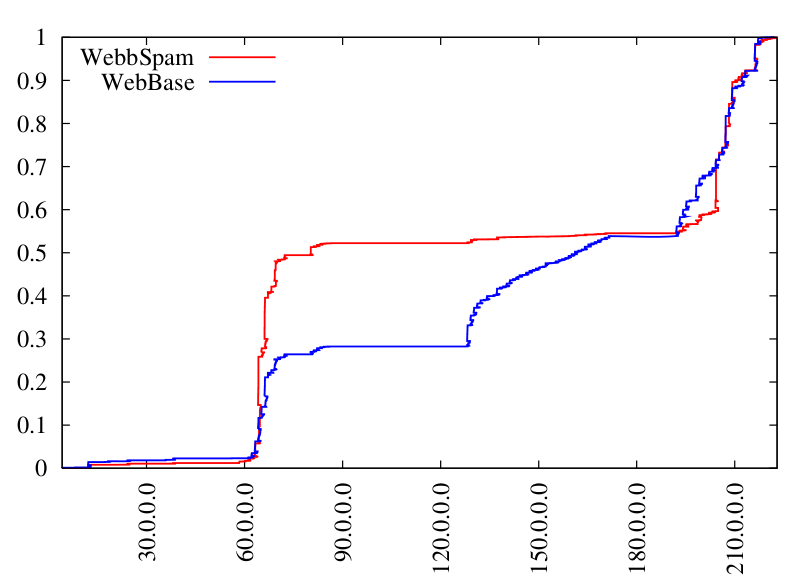
\includegraphics[width=10cm]{immagini/altre/webb.png}
\caption{Distribuzione degli indirizzi IP di due dataset: WebSpam che contiene pagine spam e WebBase che contiene pagine non spam.}
\label{img:webb1}
\end{figure}
Perciò tale metodo fa uso degli header HTTP in modo da classificare le pagine basandosi sull'osservazione che pagine spam e pagine non spam hanno valori (campi dell'header) che hanno distribuzioni distinte. Questo metodo comunque non è molto affidabile se usato da solo perciò è un ottimo strumento da usare in modo complementare ad altri metodi più tradizionali. Un uso sensato sarebbe quello di utilizzare questa tecnica come processo di preselezione in modo tale da sfoltire il numero di pagine che gli altri metodi (che si basano o sull'uso del contenuto delle pagine o del grafo del web) devono utilizzare e quindi richiedendo un numero minore di risorse.

\section{Altri metodi}
 Tra i metodi di spam detection ci sono alcuni che utilizzano pattern basati sul comportamento dell'utente per identificare le pagine spam; in \cite{Liu:2008:UBO:1367497.1367645} è illustrato un metodo che identifica le pagine spam utilizzando tre feature ricavate da pattern comportamentali che analizzano le azioni dell'utente in presenza di pagine spam e pagine non spam. Le feature sono cosi calcolate:
\begin{itemize}
 \item La prima feature è denominata SEOV (\textit{Search Engine Oriented Visit}) ed è definita come:
 \begin{equation}
  SEOV(p)=\frac{\#(Search\ engine\ oriented\ visit\ of\ p)}{\#(Visit\ of\ p)}
 \end{equation}
  dove \(p\) rappresenta la pagina web per cui viene calcolata la feature.  Il numeratore indica la visita della pagina \(p\) per mezzo dei motori di ricerca mentre il denominatore indica la visita alla pagina \(p\) senza il bisogno di utilizzare i motori di ricerca. Dato che un utente non andrebbe mai su pagine spam se non ingannato dai risultati dei motori di ricerca, le pagine spam hanno valori alti per questa feature. In figura \ref{img:seov} è rappresenta la distribuzione delle pagine (del dataset usato dagli autori) sulla base del valore della feature SEOV; in rosso sono rappresentate le pagine spam mentre in blu sono rappresentate le pagine non spam. Molte pagine web spam hanno valori SEOV più alti delle pagine non spam perché i motori di ricerca sono gli strumenti, e in alcuni casi sono gli unici, tramite cui le pagine spam possono essere raggiunte.
\begin{figure}
\centering
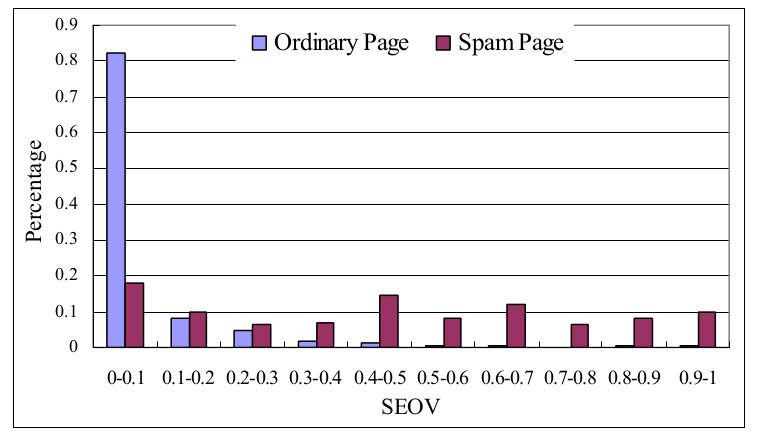
\includegraphics[width=10cm]{immagini/altre/seov.png}
\caption{Distribuzione delle pagine sulla base della feature SEOV.}
\label{img:seov}
\end{figure}
  
 \item Dal momento che esiste una grande differenza tra i contenuti di una pagina spam (ad esempio le pagine spam possono contenere molta pubblicità) e i contenuti di una pagina non spam, ci si avvale del comportamento dell'utente per etichettare le pagine. Ovvero un utente rimane su una pagina spam solo fino a al punto in cui capisce di essere su un sito con contenuti non pertinenti, mentre nel caso in cui si trovi a navigare su una pagina non spam l'utente è stimolato a rimanerci. Quindi la seconda feature è definita come SP (\textit{Start Point Visiting rate}):
 \begin{equation}
  SP(p)=\frac{\#(user\ click\ a\ hyperlink\ on\ p\ while\ visiting\ p)}{\#(Visit\ of\ p)}
 \end{equation}
 questa feature indica quanti click sono fatti su una certa pagina \(p\). In questo caso il valore al numeratore indica il numero di link cliccati dall'utente mentre naviga su una pagina \(p\); quindi ne consegue che le pagine spam avranno valori bassi rispetto alle pagine non spam.
 
 \item Infine l'ultima feature è denominata SN (\textit{Short-term Navigation rate}) e indica quante pagine di un sito \(w\) saranno visitate una volta che un utente avrà visitato tale sito \(w\). Questa misura è definita in questo modo:
 \begin{equation}
  SN(w)=\frac{\#(Session\ in\ wich\ users\ visit\ less\ than\ N\ pages\ in\ w)}{\#(Session\ in\ wich\ user\ visit\ w)}
 \end{equation}
 \end{itemize}
La novità di questo metodo sta nel fatto che mentre gli altri metodi sono basati sullo studio di determinate proprietà che le pagine web hanno o sullo studio del grafo del web  (quindi la tipologia che le pagine web assumo all'interno del grafo) quest'ultimo metodo si basa sul comportamento dell'utente. Quindi tale metodo utilizzando pattern comportamentali per determinare le pagine spam è molto più flessibile dei metodi tradizionali, i quali sono dipendenti dalla struttura della pagina o del grafo.
A differenza  dei metodi classici che si basano su delle euristiche riscontrate su alcuni dataset e quindi sono dipendenti dalla tipologia di spam che si riscontra perciò non sono flessibili in modo da rilevare nuovi tipi di tecniche spam, questo ultimo metodo rende il problema dell'identificazione dello spam scalabile, ovvero potrebbe riuscire a rilevare anche le nuove tipologie di spam web che potrebbero essere implementate. 

Un altro metodo che fanno uso del comportamento dell'utente durante la navigazione web per determinare le pagine spam è \textit{BrowseRank} \cite{Liu:2008:BLW:1390334.1390412}. \textit{BrowseRank} determina l'importanza di una pagina web utilizzando il grafo ricavato dal comportamento dell'utente durante la navigazione web con attraverso il browser. Il grafo è costituito da vertici che rappresentano le pagine. da archi orientati che rappresentano le transizioni da una pagina all'altra da parte dell'utente e anche dal tempo di permanenza su una pagina. Infine come per \textit{Pagerank} viene utilizzato il grafo ricavato per determinare l'importanza delle pagine.\\
In figura \ref{img:browser} è rappresentato uno schema esplicativo del modo con cui si ricava il grafo. Il grafo è ricavato dai browser degli utenti (ad esempio tramite l'utilizzo di toolbar) che raccolgono diversi dati come l'URL, il tempo di permanenza, la tipologia della visita (ad esempio se l'utente ha inserito l'URL nella barra degli indirizzi 
del browser oppure se arrivato a ad una pagina per mezzo di un link) e vengono poi recuperati da un server che integra i dati provenienti da milioni di utenti.
\begin{figure}
\centering
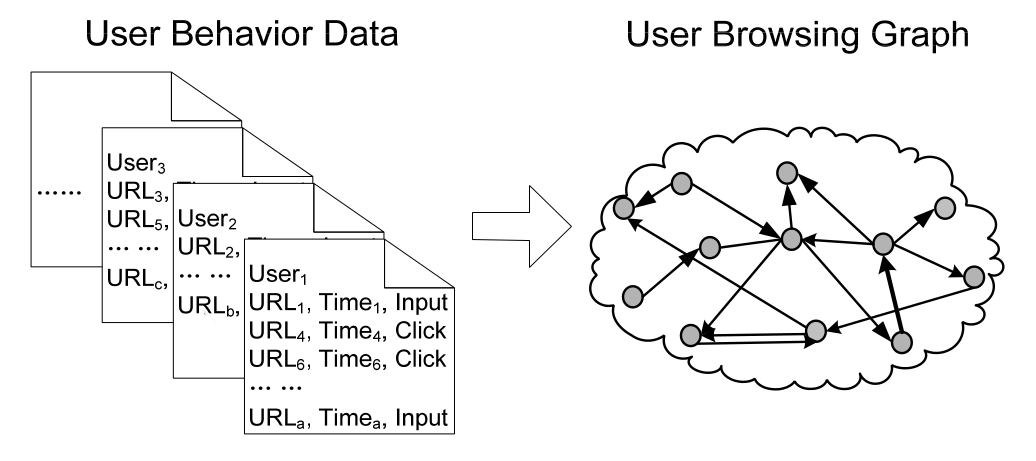
\includegraphics[width=10cm]{immagini/altre/browser.png}
\caption{Dal comportamento dell'utente al grafo.}
\label{img:browser}
\end{figure}
Questo algoritmo ha due vantaggi principali rispetto ai metodi tradizionali sui link quali:
\begin{itemize}
 \item Dato che il grafo è ricavato durante la fase di navigazione è più accurato di quello ricavato da un crawler perché i link tra le pagine possono cambiare continuamente.
 \item Inoltre tale metodo tiene conto anche del tempo in cui ci si sofferma su una pagina; questa caratteristica può fare capire se si è in presenza di una pagina spam: infatti un utente non avrebbe nessun vantaggio a rimanere a lungo su una pagina con poca pertinenza e qualità rispetto al suo bisogna di informazione.
\end{itemize}
\newpage
Dagli esperimenti gli autori hanno notato che \textit{BrowseRank} è più efficiente rispetto a \textit{Trustrank} e quindi dimostra che i metodi che si basano su segnali differenti dal contenuto o dal grafo del web possono essere in grado di lavorare autonomamente e non solo in modo  complementare ai metodi classici.


